\documentclass[14pt]{extbook}
\usepackage{multicol, enumerate, enumitem, hyperref, color, soul, setspace, parskip, fancyhdr} %General Packages
\usepackage{amssymb, amsthm, amsmath, latexsym, units, mathtools} %Math Packages
\everymath{\displaystyle} %All math in Display Style
% Packages with additional options
\usepackage[headsep=0.5cm,headheight=12pt, left=1 in,right= 1 in,top= 1 in,bottom= 1 in]{geometry}
\usepackage[usenames,dvipsnames]{xcolor}
\usepackage{dashrule}  % Package to use the command below to create lines between items
\newcommand{\litem}[1]{\item#1\hspace*{-1cm}\rule{\textwidth}{0.4pt}}
\pagestyle{fancy}
\lhead{Progress Quiz 4}
\chead{}
\rhead{Version B}
\lfoot{5346-5907}
\cfoot{}
\rfoot{Summer C 2021}
\begin{document}

\begin{enumerate}
\litem{
Solve the linear equation below. Then, choose the interval that contains the solution.\[ \frac{3x -7}{3} - \frac{-3x + 5}{8} = \frac{4x + 9}{5} \]\begin{enumerate}[label=\Alph*.]
\item \( x \in [3.1, 8.1] \)
\item \( x \in [35.52, 40.52] \)
\item \( x \in [1.38, 3.38] \)
\item \( x \in [7.28, 10.28] \)
\item \( \text{There are no real solutions.} \)

\end{enumerate} }
\litem{
Solve the equation below. Then, choose the interval that contains the solution.\[ -6(18x -19) = -17(15x -4) \]\begin{enumerate}[label=\Alph*.]
\item \( x \in [0.61, 2.22] \)
\item \( x \in [-0.62, 0.21] \)
\item \( x \in [-0.07, 0.74] \)
\item \( x \in [-1.89, -1.23] \)
\item \( \text{There are no real solutions.} \)

\end{enumerate} }
\litem{
First, find the equation of the line containing the two points below. Then, write the equation in the form $ y=mx+b $ and choose the intervals that contain $m$ and $b$.\[ (9, -4) \text{ and } (5, 9) \]\begin{enumerate}[label=\Alph*.]
\item \( m \in [-1.75, 6.25] \hspace*{3mm} b \in [-11.25, -5.25] \)
\item \( m \in [-4.25, -2.25] \hspace*{3mm} b \in [-18, -8] \)
\item \( m \in [-4.25, -2.25] \hspace*{3mm} b \in [-1, 8] \)
\item \( m \in [-4.25, -2.25] \hspace*{3mm} b \in [-33.25, -24.25] \)
\item \( m \in [-4.25, -2.25] \hspace*{3mm} b \in [24.25, 31.25] \)

\end{enumerate} }
\litem{
Write the equation of the line in the graph below in Standard Form $Ax+By=C$. Then, choose the intervals that contain $A, B, \text{ and } C$.
\begin{center}
    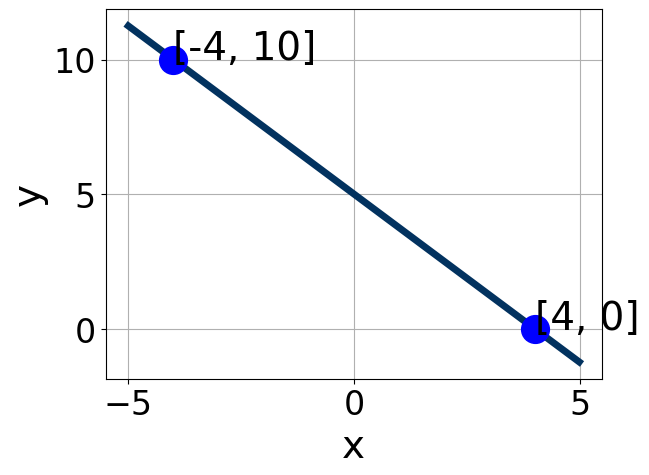
\includegraphics[width=0.5\textwidth]{../Figures/linearGraphToStandardCopyB.png}
\end{center}
\begin{enumerate}[label=\Alph*.]
\item \( A \in [4.7, 7.3], \hspace{3mm} B \in [2.94, 4.93], \text{ and } \hspace{3mm} C \in [18, 26] \)
\item \( A \in [-0.2, 2.9], \hspace{3mm} B \in [0.43, 1.51], \text{ and } \hspace{3mm} C \in [-1, 6] \)
\item \( A \in [-0.2, 2.9], \hspace{3mm} B \in [-2.57, 0.34], \text{ and } \hspace{3mm} C \in [-9, -2] \)
\item \( A \in [-8.8, -4.1], \hspace{3mm} B \in [-4.81, -3.18], \text{ and } \hspace{3mm} C \in [-20, -17] \)
\item \( A \in [4.7, 7.3], \hspace{3mm} B \in [-4.81, -3.18], \text{ and } \hspace{3mm} C \in [-20, -17] \)

\end{enumerate} }
\litem{
Find the equation of the line described below. Write the linear equation in the form $ y=mx+b $ and choose the intervals that contain $m$ and $b$.\[ \text{Perpendicular to } 6 x + 7 y = 8 \text{ and passing through the point } (6, 8). \]\begin{enumerate}[label=\Alph*.]
\item \( m \in [0.24, 0.9] \hspace*{3mm} b \in [0.27, 1.74] \)
\item \( m \in [-1.49, -0.49] \hspace*{3mm} b \in [14.55, 16.43] \)
\item \( m \in [1.03, 1.47] \hspace*{3mm} b \in [0.27, 1.74] \)
\item \( m \in [1.03, 1.47] \hspace*{3mm} b \in [-1.21, -0.14] \)
\item \( m \in [1.03, 1.47] \hspace*{3mm} b \in [1.71, 2.97] \)

\end{enumerate} }
\litem{
Solve the equation below. Then, choose the interval that contains the solution.\[ -19(7x -12) = -2(11x -5) \]\begin{enumerate}[label=\Alph*.]
\item \( x \in [-2.29, -2.1] \)
\item \( x \in [2.13, 2.41] \)
\item \( x \in [1.91, 2.08] \)
\item \( x \in [1.43, 1.61] \)
\item \( \text{There are no real solutions.} \)

\end{enumerate} }
\litem{
Find the equation of the line described below. Write the linear equation in the form $ y=mx+b $ and choose the intervals that contain $m$ and $b$.\[ \text{Perpendicular to } 8 x - 7 y = 10 \text{ and passing through the point } (2, -2). \]\begin{enumerate}[label=\Alph*.]
\item \( m \in [-1, -0.2] \hspace*{3mm} b \in [-4.1, -3.8] \)
\item \( m \in [0.4, 1] \hspace*{3mm} b \in [-3.88, -3.55] \)
\item \( m \in [-1, -0.2] \hspace*{3mm} b \in [-0.03, 0.46] \)
\item \( m \in [-1, -0.2] \hspace*{3mm} b \in [-0.3, 0.01] \)
\item \( m \in [-2.3, -1] \hspace*{3mm} b \in [-0.3, 0.01] \)

\end{enumerate} }
\litem{
Write the equation of the line in the graph below in Standard Form $Ax+By=C$. Then, choose the intervals that contain $A, B, \text{ and } C$.
\begin{center}
    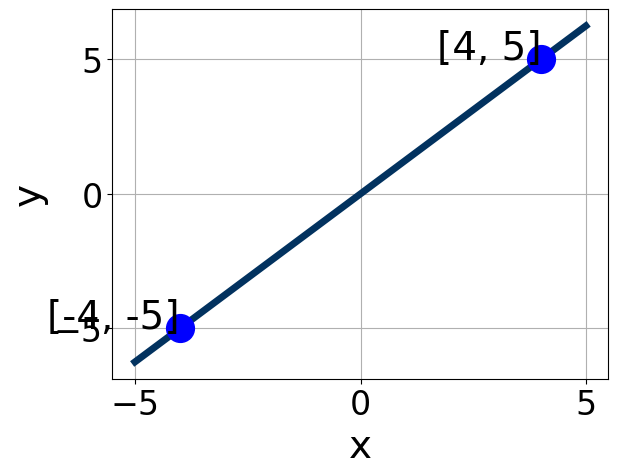
\includegraphics[width=0.5\textwidth]{../Figures/linearGraphToStandardB.png}
\end{center}
\begin{enumerate}[label=\Alph*.]
\item \( A \in [4, 7.2], \hspace{3mm} B \in [-4.7, -3.4], \text{ and } \hspace{3mm} C \in [-1, 7] \)
\item \( A \in [-5.9, -3.7], \hspace{3mm} B \in [3.6, 6.8], \text{ and } \hspace{3mm} C \in [-1, 7] \)
\item \( A \in [-2.1, 2.8], \hspace{3mm} B \in [-1.7, -0.2], \text{ and } \hspace{3mm} C \in [-1, 7] \)
\item \( A \in [4, 7.2], \hspace{3mm} B \in [3.6, 6.8], \text{ and } \hspace{3mm} C \in [-1, 7] \)
\item \( A \in [-2.1, 2.8], \hspace{3mm} B \in [-0.3, 2.7], \text{ and } \hspace{3mm} C \in [-1, 7] \)

\end{enumerate} }
\litem{
Solve the linear equation below. Then, choose the interval that contains the solution.\[ \frac{-7x -6}{3} - \frac{-9x -4}{4} = \frac{-7x + 8}{5} \]\begin{enumerate}[label=\Alph*.]
\item \( x \in [3.1, 5.8] \)
\item \( x \in [1.6, 2.2] \)
\item \( x \in [-0.1, 0.3] \)
\item \( x \in [6.9, 8] \)
\item \( \text{There are no real solutions.} \)

\end{enumerate} }
\litem{
First, find the equation of the line containing the two points below. Then, write the equation in the form $ y=mx+b $ and choose the intervals that contain $m$ and $b$.\[ (8, -11) \text{ and } (6, 9) \]\begin{enumerate}[label=\Alph*.]
\item \( m \in [-14, -1] \hspace*{3mm} b \in [2, 8] \)
\item \( m \in [6, 11] \hspace*{3mm} b \in [-52, -48] \)
\item \( m \in [-14, -1] \hspace*{3mm} b \in [-21, -12] \)
\item \( m \in [-14, -1] \hspace*{3mm} b \in [66, 73] \)
\item \( m \in [-14, -1] \hspace*{3mm} b \in [-73, -68] \)

\end{enumerate} }
\end{enumerate}

\end{document}